
\section{跳过或更改坐标——过滤器}
\label{sec:filters}

\PGFPlots{} 提供过滤器。过滤器接受一个（数值）输入坐标，并允许修改该坐标或将其丢弃。过滤器可以单独作用于各个坐标，也可以同时作用于所有坐标。一个主要应用是跳过坐标，即安装一个导致坐标被跳过的过滤器。这通过分配特殊的“此坐标不存在”值来代替原始值来实现。“此坐标不存在”的有效选项使用 |unbounded coords| 定义，如 Section~\ref{sec:pgfplots:interrupt}（关于中断的图）所述，即 |empty line| 或 |unbounded coords|。

有关不同类型的变换及其相互作用，另请参见 Section~\ref{sec:transformation:interaction}。

\begin{pgfplotsxyexpressionkeylist}{\x\space filter}
    安装一个坐标过滤器，允许修改\emph{单个}坐标的当前值。

    参数\emph{math expression}是一个包含 |x|、|y| 或 |z| 的数学表达式。
    %
\begin{codeexample}[]
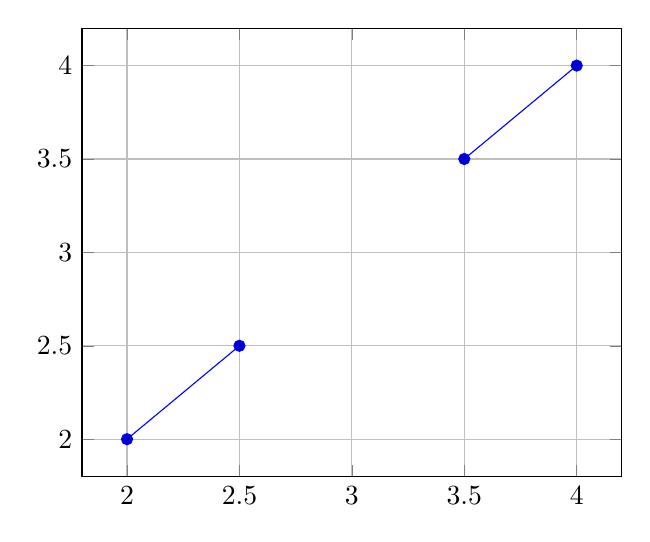
\begin{tikzpicture}
\begin{axis}[grid=major]
    \addplot+ [
        unbounded coords=jump,
        x filter/.expression={x+1},
        y filter/.expression={y==3 ? nan : y},
    ] table {
        x   y
        1   2
        1.5 2.5
        2   3
        2.5 3.5
        3   4
    };
\end{axis}
\end{tikzpicture}
\end{codeexample}

    |x filter| 最先求值。它可以依赖于 |x|、|y| 和 |z|，它们的值是“预处理过的”坐标：即应用 |x coord trafo| 和任何对数（对于对数坐标轴）之后得到的值。

    |y filter| 接着求值。它可以依赖于 |x|，即 |x filter| 的结果。它也可以依赖于 |y| 和 |z|，它们的值与上一段讨论的相同。

    |z filter| 最后求值。它可以依赖于 |x| 和 |y|，即它们各自过滤器的结果。它也可以依赖于 |z|，即普通的 $z$ 坐标（如 |x filter| 所讨论的）。

    请注意，过滤器值可以包含可展开材料，包括用于表格的 |\thisrow|：
    %
\begin{codeexample}[]
\begin{tikzpicture}
\begin{axis}
    \addplot+[
        x filter/.expression={
            \thisrow{W} == 42 ? 0.2 : x
        },
    ] table {
        x y     W
        0 0     41
        0.5 0.5 42
        1 1     43
    };
\end{axis}
\end{tikzpicture}
\end{codeexample}
    %
    通过数学表达式定义过滤器实际上是 |x filter| 的一个特例，见下文。因此，\meta{expression} 可以包含 |\pgfmathresult|，即未修改的输入值（参见下面 |x filter| 的说明）。
\end{pgfplotsxyexpressionkeylist}

\begin{pgfplotsxyappendexpressionkeylist}{\x\space filter}
    这些是 |x filter/.expression| 的变体，允许\emph{追加}另一个坐标过滤器。在这种情况下，你可以为同一坐标设置不同的过滤器，每个都基于前一个过滤器的输出：
    %
\begin{codeexample}[]
\begin{tikzpicture}
\begin{axis}
    \addplot+[
        y filter/.append expression={
            abs(x-1) < 1e-4 ? 1.5 : \pgfmathresult
        },
        y filter/.append expression={
            abs(x-3) < 1e-4 ? NaN : \pgfmathresult
        },
    ] table {
        x y
        0 0
        1 1
        2 2
        3 3
        4 4
    };
\end{axis}
\end{tikzpicture}
\end{codeexample}
    %
    该示例安装了两个 |y filter|：第一个检查 $x = 1$，在此情况下定义 $y=1.5$，否则它告诉过滤器“使用过滤器之前的 $y$ 值”。第二个过滤器检查 $x = 3$，如果是则分配值“Not a Number”（这会丢弃该坐标）。否则它告诉过滤器“使用过滤器之前的 $y$ 值”，即由\emph{第一个}过滤器生成的值。

    如你所见，特殊宏“|\pgfmathresult|”始终产生未修改的输入值。这是底层 |x filter| 功能的一个特性。

    请注意，该示例可以通过将第一个“|\pgfmathresult|”替换为“|y|”来改写。但为了简化复制/粘贴，以始终增量的方式表述增量过滤器是有意义的。

    如果之前没有其他过滤器，安装 |x filter/.append expression| 与 |x filter/.expression| 相同。即使已有某个自定义 |x filter|（例如用下面概述的 |x filter/.code| 安装的），“append”功能也会应用。因此，“append”的语义是“追加另一个坐标过滤器”，而不是“向现有表达式追加另一个表达式”。唯一的要求是前一个过滤器不得用空值替换坐标。静默丢弃值并返回空值的过滤器必须追加在 |.append expression| 之后。
\end{pgfplotsxyappendexpressionkeylist}

\begin{pgfplotsxycodekeylist}{\x\ filter,filter point}
    代码键 |x filter| 和 |y filter| 是 |x filter/.expression| 及其变体的高级变体。它们允许修改\emph{单个}坐标值，但可以执行任意 \TeX{} 代码。坐标过滤器以 |#1| 作为输入坐标（输入时，相同的值存储在 |\pgfmathresult| 中），应用某些操作并将结果写入宏 |\pgfmathresult|。如果之后 |\pgfmathresult| 为空，则该坐标被丢弃。你也可以将 |\pgfmathresult| 设置为 |nan| 或 |inf|，在这种情况下，该坐标要么被丢弃（如果设置了 |unbounded coords=discard|），要么图可以被中断（即 |unbounded coords=jump| 的情况）。

    |filter point/.code| 过滤器允许根据构成完整点的所有分量（$x$、$y$ 和 $z$）进行过滤；见下文。

    过滤器可以不更改 |\pgfmathresult|。在这种情况下，将使用未过滤的坐标。

    坐标过滤器在自动处理系统中很有用，其中 \PGFPlots{} 用于显示自动生成的图。你可能不想手动过滤坐标，因此这些选项提供了自动执行此操作的工具。

    下面的过滤器为每个 $x$ 坐标加上 $0.5$。
    %
\begin{codeexample}[]
\begin{tikzpicture}
\begin{axis}[
    % equivalent to 'x filter/.expression={x+0.5}'
    x filter/.code={
        \pgfmathadd{#1}{0.5}
    },
]
    \addplot coordinates {
        (4,0)
        (6,1)
    };
\end{axis}
\end{tikzpicture}
\end{codeexample}
    %
    有关 \PGF{} 数学引擎的详细信息，请参见~\cite[pgfmath manual]{tikz}。只要可能，基于数学的过滤器应使用 |x filter/.expression| 表述，因为这会降低复杂性并确保最佳精度（它也适用于 |lua backend|）。

    在过滤器求值期间，宏 |\coordindex| 包含当前坐标的编号（从~$0$ 开始）。因此，下面的过滤器丢弃第 $5$ 个之后和第 $10$ 个之前的所有坐标。
    %
\begin{codeexample}[]
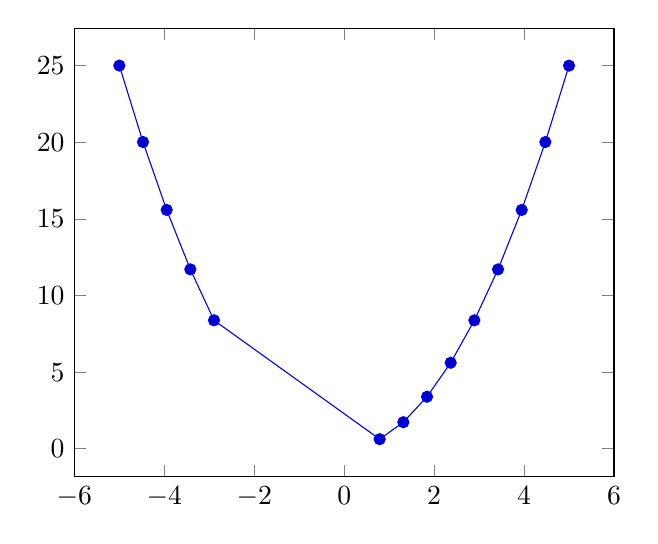
\begin{tikzpicture}
\begin{axis}[
    samples=20,
    % equivalent to
    % x filter/.expression={
    %   \coordindex>4 && \coordindex<11 ? nan : x
    % },
    x filter/.code={
        \ifnum\coordindex>4
            \ifnum\coordindex<11
                \def\pgfmathresult{}
            \fi
        \fi
    },
]
    \addplot {x^2};
\end{axis}
\end{tikzpicture}
\end{codeexample}
    %
    还有一个样式键简化按索引选择，见下文。

    \PGFPlots{} 调用过滤器时，参数 |#1| 设置为输入坐标。对于 $x$ 过滤器，这是指定给 |\addplot| 的 $x$ 坐标；对于 $y$ 过滤器，它是 $y$ 坐标。

    如果相应的坐标轴是对数坐标轴，|#1| 是该坐标的\emph{对数}（参见 |log basis x| 及其变体）作为实数，例如 |#1=4.2341|。如果对数未定义，该参数将为空。

    坐标过滤器的参数经过最少的预处理：首先，对于对数坐标轴，提供参数的\emph{对数}。其次，应用任何高级坐标映射，如 |x coord trafo|（可用于将日期映射为数字或将字符串映射为数字等）。因此，|#1| 参数应为数字。未应用进一步的变换。

    偶尔，获取坐标输入例程报告的“原始”、完全未处理的输入坐标可能很方便。此未处理数据在三个数学解析器常量 \declareandlabel{rawx}、\declareandlabel{rawy} 和 \declareandlabel{rawz} 中可用。所有这些值都可直接用于过滤器（一些其他方法也会影响图）。请注意，|rawy| 应像无参数函数一样使用，即在进行数学解析的地方过滤器可以使用它。

    一个应用可以是基于正常刻度过滤对数值：
    %
\begin{codeexample}[]
\begin{tikzpicture}
\begin{semilogyaxis}
    \addplot+ [
        restrict expr to domain={rawy}{1e0:1.5e1},
    ] {exp(x)};
\end{semilogyaxis}
\end{tikzpicture}
\end{codeexample}
    %
    \noindent 前面的示例使用 |rawy| 将范围 $[1,15]$ 之外的所有样本丢弃。

    如果对 |\addplot table| 调用键过滤器，可以使用 |\thisrow|\marg{column name}（及其变体）访问当前行的数据。这包括表格的所有列。

    |filter point| 键更具技术性。它不接受参数：其参数以 |pgfkeys| 变量 |/data point/x|、|/data point/y| 和 |/data point/z| 的形式给出。它可以使用 |\pgfkeyssetvalue{/data point/x}|\marg{new value} 更改其坐标；可以使用 |\pgfkeysvalueof{/data point/x}| 访问变量，或者如果参数应写入宏，则使用 |\pgfkeysgetvalue|。此过滤器在其他过滤器之后求值。

    请注意，你可以为每个 |\addplot| 命令提供不同的 |x filter|/|y filter| 参数。似乎只有 `|#1|' 参数有问题，我还没有查明原因。如果你提供 |\addplot[x filter/.code={...}]|，请使用 |\pgfmathresult| 代替 |#1|。

    请注意，坐标过滤也适用于 |mesh|、|surf| 和 |patch| 图。\index{mesh!Coordinate filtering}\index{surf!Coordinate filtering}在此上下文中，当且仅当某个 |patch type| 的所有顶点都有有界坐标时才绘制它。换句话说：如果一个矩形（比方说）的一个顶点被过滤掉，整个矩形将被省略。|mesh| 和 |surf|ace 图的坐标过滤还有一个特殊要求：此类图的默认值为 |mesh input=lattice|。如果坐标过滤器静默丢弃一个坐标，晶格将断裂，\PGFPlots{} 会变得混乱。因此，|mesh| 和 |surf|ace 图的坐标过滤始终需要 |unbounded coords=jump|，任何被过滤掉的点应接收值 |nan| 而非空字符串（因为即使在 |unbounded coords=jump| 存在的情况下，空字符串也\emph{始终}被丢弃）。有关坐标过滤和三维图的详细信息，请参见 |unbounded coords| 的参考文档及其中第~\pageref{sec:pgfplots:interrupt} 页的示例。
\end{pgfplotsxycodekeylist}

\begin{pgfplotscodekey}{pre filter}
    在 |x filter|、|y filter| 和 |z filter| 之前应用。
\end{pgfplotscodekey}

\begin{stylekey}{/pgfplots/skip coords between index=\marg{begin}\marg{end}}
    一个追加 |x filter| 的样式，该过滤器丢弃选定的坐标。选择按索引进行，索引从~$0$ 开始，参见 |\coordindex|。每个索引满足 $\mathit{begin} \le i < \mathit{end}$ 的坐标都将被跳过。
    %
\begin{codeexample}[]
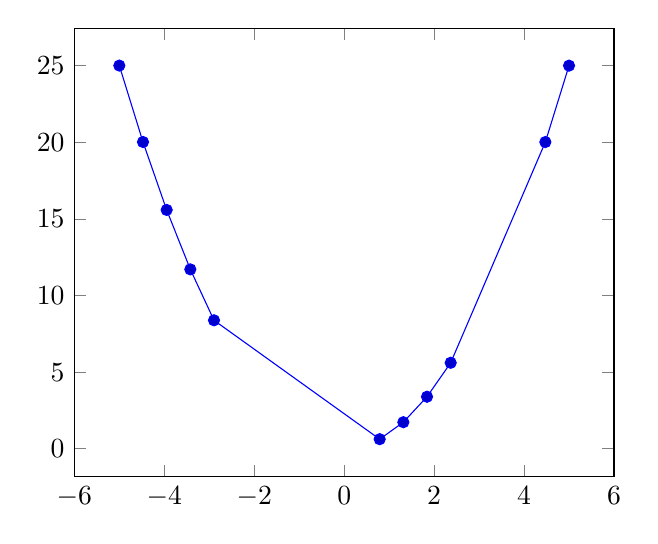
\begin{tikzpicture}
\begin{axis}[
    samples=20,
    skip coords between index={5}{11},
    skip coords between index={15}{18},
]
    \addplot {x^2};
\end{axis}
\end{tikzpicture}
\end{codeexample}

    \paragraph{技术说明：}

    此样式通常应用于 $x$ 坐标（即它计数 $x$ 坐标）。如果你想将其应用于类似 |hist/data| 或 |quiver/u| 的内容，可以
    %
    \begin{enumerate}
        \item 在样式名称后追加星号 `|*|'，并
        \item 将目标坐标名称作为第一个参数提供。
    \end{enumerate}
    %
    例如，|skip coords between index*={hist/data}{2}{4}| 应用于 |hist/data|。
\end{stylekey}

\begin{pgfplotskey}{each nth point=\marg{integer}}
    一个追加 |x filter| 的样式，该过滤器丢弃除每第 $n$ 个输入坐标之外的所有坐标。\index{Downsampling}

    这种降采样效果相当好。它可用于减少输入文件中的大量坐标。在这种情况下，你还应设置 |filter discard warning=false| 以避免关于跳过坐标的重复通知，并设置 |unbounded coords=discard|，使 \PGFPlots{} 静默地遗忘任何丢弃的点（而非生成中断的图）。

    请注意，还有一个 |mark repeat| 样式，它仅对绘图标记应用相同的操作。


    \paragraph{技术说明：}

    此样式通常应用于 $x$ 坐标（即它计数 $x$ 坐标）。如果你想将其应用于类似 |hist/data| 或 |quiver/u| 的内容，可以
    %
    \begin{enumerate}
        \item 在样式名称后追加星号 `|*|'，并
        \item 将目标坐标名称作为第一个参数提供。
    \end{enumerate}
    %
    例如，|each nth point*={hist/data}{2}{4}| 应用于 |hist/data|。
\end{pgfplotskey}

\begin{pgfplotsxykeylist}{%
    restrict \x\space to domain=\meta{min}:\meta{max},
    restrict \x\space to domain*=\meta{min}:\meta{max}%
}
\labelprefix\label{key:restrict:x:to:domain}
    这些键追加 $x$（或 $y$ 或 $z$）坐标过滤器，将相应坐标限制在某个定义域内。

    \tikzset{external/figure name/.add={}{restrictodomain_}}%

    不带星号的版本（如 |restrict x to domain|）会在坐标低于 \meta{min} 时分配值 |-inf|，在坐标高于 \meta{max} 时分配 |+inf|。带星号的版本（如 |restrict x to domain*|）会将坐标截断到 $[\mathit{min}, \mathit{max}]$，即如果坐标落在下限之外，它们分配值 \meta{min}；如果值落在上限之外，则分配 \meta{max}。

    对于对数坐标轴，\meta{min} 和 \meta{max} 是相应值的\emph{对数}。使用非对数数字的一个变体可以是使用 |restrict expr to domain={\pgfmathrawx}|\marg{min}\marg{max}。

    不带星号的版本还设置 |unbounded coords=jump|，这会导致中断的图。
    %
\pgfplotsexpensiveexample
\begin{codeexample}[]
\begin{tikzpicture}
    \begin{axis}[
        restrict y to domain=-10:10,
        samples=1000,
        % some fine-tuning for the display:
        width=10cm, height=210pt,
        xmin=-4.7124, xmax=4.7124,
        xtick={-4.7124,-1.5708,...,10},
        xticklabels={$-\frac32 \pi$,$-\pi/2$,$\pi/2$,$\frac32 \pi$},
        axis x line=center,
        axis y line=center,
    ]
        \addplot [blue] gnuplot [id=tangens,domain=-1.5*pi:1.5*pi] {tan(x)};
        \legend{$\tan(x)$}
    \end{axis}
\end{tikzpicture}
\end{codeexample}
\end{pgfplotsxykeylist}

\begin{pgfplotskeylist}{%
    restrict expr to domain=\marg{expression}\marg{\meta{min}:\meta{max}},
    restrict expr to domain*=\marg{expression}\marg{\meta{min}:\meta{max}}%
}
    追加一个 $x$ 坐标过滤器，如果 \meta{expression} 求值为小于 \meta{min} 的值，则将 $x$ 坐标设置为 |-inf|；如果 \meta{expression} 求值为大于 \meta{max} 的值，则设置为 |inf|。

    带星号的变体 |restrict to domain*| 在 \meta{expression} 小于下限时分配 \meta{min}，在大于上限时分配 \meta{max}。

    不带星号的版本还设置 |unbounded coords=jump|，这会导致中断的图。

    与 |restrict x to domain| 不同，\meta{expression} 可以依赖于 |\addplot| 期间有效的任何内容，特别是 |\coordindex| 或表格列（|\thisrow|\marg{column name} 等）。该表达式完全不需要依赖 $x$。
\end{pgfplotskeylist}

\begin{pgfplotskey}{%
    @restrict to domain=\marg{filter name}\marg{expression}\marg{\meta{min}:\meta{max}}\mchoice{0,1}%
}
    一个底层（技术）键，允许将 |restrict * to ...| 功能也应用于类似 |hist/data| 的内容。

    例如，|@restrict to domain={hist/data}{}{0:1}{0}| 将定义域限制应用于直方图输入 |hist/data|。最后的 `|0|' 表示它的工作方式与键 |restrict x to domain=0:1| 类似，即它跳过 $[0,1]$ 之外的所有内容。类似地，|@restrict to domain={hist/data}{}{0:1}{1}| 将 |restrict x to domain*=0:1| 的功能应用于 |hist/data|：它将 $[0,1]$ 之外的值截断到定义域的端点。

    \meta{filter name} 应为坐标名，如 |x|、|y|、|z|（或 |hist/data|）。

    \meta{expression} 配置一个表达式，将使用它而非 \meta{filter name} 的值。它可以为空。

    \meta{min}\texttt{:}\meta{max} 如上所述。

    如果最后一个参数是 |1|，允许定义域之外的任何坐标将以定义域边界作为值。如果是 |0|，这样的坐标将获得 |inf| 或 |-inf|。
\end{pgfplotskey}

\begin{pgfplotskey}{filter discard warning=\mchoice{true,false} (initially true)}
    每当坐标过滤器丢弃坐标时，在日志文件中发出通知。
\end{pgfplotskey}

你可以在 Section~\ref{sec:pgfplots:interrupt}：“中断的图”中找到更多关于坐标过滤的内容。
